In this section, we describe our experimental study of the methods mentioned or proposed in the chapter, which serves two purposes: (1) demonstrating the performance of our fast computational methods, and (2) characterizing the solution structure of \prob under different problem settings.
%

The algorithms are implemented in C++ and run on a 3.6GHz quad-core CPU with 16G memory.
For integer linear programming, Gurobi \cite{optimization2019gurobi} is used as the solver with a time limit of 60 seconds applied.
In the evaluation, two main factors are considered: computation time and solution quality measured by interception rate. 

The instances were generated for up to dozens of defenders, 
and the defender speeds are sampled uniformly at random from $1$ to $v_{max}$.
The attack sequence was generated according to a Poisson process with parameter $\lambda$ (i.e., the time gap between
two consecutive attacks conforms with an exponential distribution $P(t) = \lambda e^{-\lambda t}$),
and the locations of the attack are sampled uniformly at random from the boundary.
We use 4 types of boundary for testing a) unit circle $S^1$, b) unit interval $I=[0, 1]$
c) unit square $I^2=[0, 1]\times[0,1]$, and d) unit sphere $S^2$.

\subsection{Infinite-Horizon \prob: Basic Performance Evaluation}
This section provides experimental study and comparisons between the three methods described in the section: 
dynamic programming (DP), integer linear programming (ILP), and exhaustive defender pairing (\ours) algorithms.
% \subsubsection{Computation time}

To test and compare the general performance of these methods, we set the defending task on $S^1$ (i.e., a circular boundary with a distance of $2\pi$) 
with the attack sequence's coming rate $\lambda$ (used in the Poisson process) proportional to $k$, the number of defenders. 
The results on computational time and interception rate are given in Figs.~\ref{fig:bd-time_cost} and~\ref{fig:bd-quality}.

\begin{figure}[h!]
    \centering
    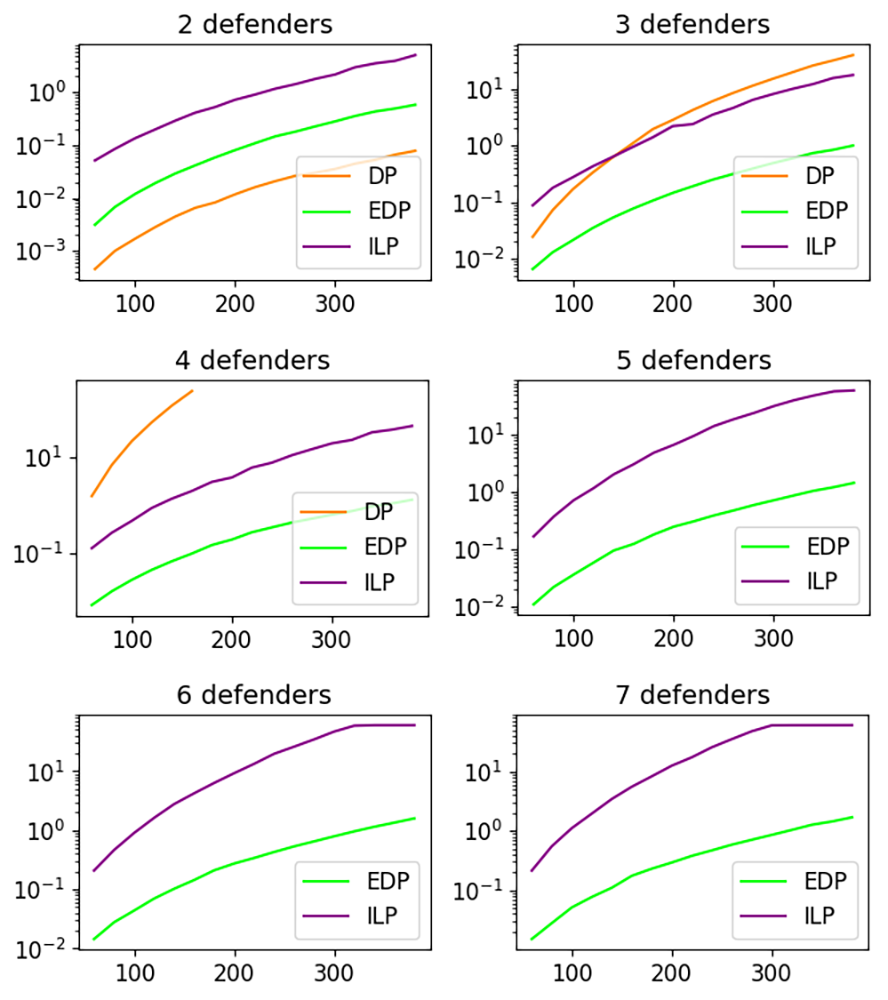
\includegraphics[width=.5\linewidth]{chapters/bd/fig/timecost-v.png}
    \caption[Computation time for DP, ILP and \our]{Computation time in seconds ($y$-axis) for dynamic programming (DP), integer linear programming (ILP) and \ours for 2 to 7 defenders and up to 400 attack events ($x$-axis). DP quickly becomes intractable as the number of defenders goes beyond $3$; ILP is about 2-3 magnitudes slower than \ours.}
    \label{fig:bd-time_cost}
\end{figure}

% \subsubsection{Solution quality}

\begin{figure}[h!]
    \centering
    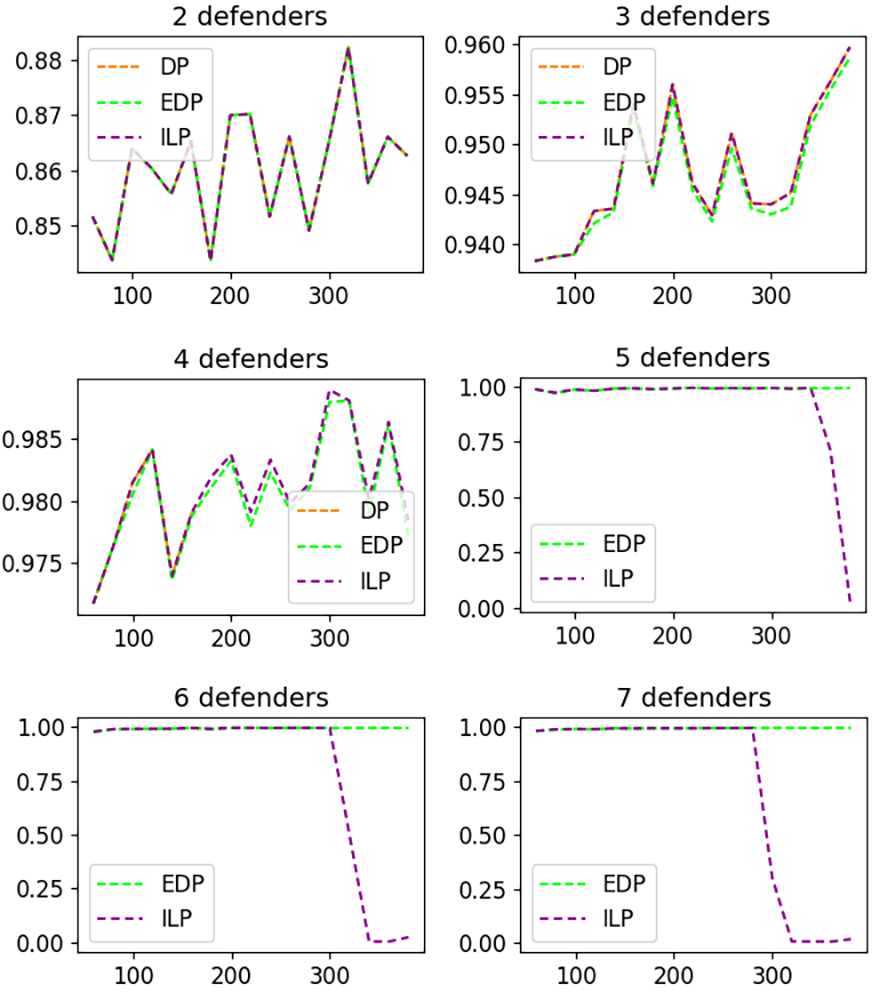
\includegraphics[width=.5\linewidth]{chapters/bd/fig/quality-v.png}
    \caption[Solution quality for DP, ILP and \our]{Solution quality (interception rate) for dynamic programming (DP), integer linear programming (ILP) and \ours  for 2 to 7 defenders. For all settings, \ours achieves optimality nearly identical to the optimal DP and ILP (when DP and ILP can complete the computation). ILP starts to fail as the number of defenders reaches $5$ and the number of events exceeds $300$.}
    \label{fig:bd-quality}
\end{figure}

For 2 to 7 defenders, in ~\ref{fig:bd-time_cost}, we show the computation time of running the algorithms. 
Each data point is an average of 20 runs. 
We remind the readers that both DP and ILP guarantee to produce an optimal solution (if they can finish).
For the two-defender scenario, which is the main focus of \cite{adler2022role}, DP is the most efficient.
However, DP only fully scales for $k=2, 3$ defenders, and start to peter out for $k=4$ defenders due to memory limit (so its running time is not shown for $k>4$).
%The integer programming method was set a time limit of 60s for solving the model.
As can be observed, ILP demonstrates much better scalability in comparison to DP, but fails to find a solution for $k > 5$ defenders. 

As expected, exhaustive defender pairing (\ours) has the least time cost for $k \geq 3$.
~\ref{fig:bd-quality} shows the corresponding solution qualities of these methods. 
We observe that, while \ours does not guarantee solution optimality, it generated solutions that are virtually the same as the exact methods (DP and ILP). 
%
Through these empirical evaluations, \ours demonstrates superior scalability with negligible solution optimality loss. 

%\textbf{JJ's edit location}


\subsection{Scaling up the Number of Defenders}
The number of defenders appears in the index term of the time complexity of the DP algorithm, which limits it from scaling up the number of defenders. Hence, we compare the performance of ILP and the local search algorithm when pushing the number of defenders up to dozens. With the main goal being the evaluation of optimality, we limit the attack events to $200$ so that the ILP method can return the optimal solution in $60$ seconds. At the same time, to make the problem more challenging, 
$\lambda$ is increased to $2\cdot k$ from $k$ so that not all attacks can be intercepted. 
~\ref{fig:bd-def_time_cost} and  ~\ref{fig:bd-def_quality} show the corresponding computation time 
and interception rate, each data point is the average of 20 runs.

\begin{figure}[h!]
    \centering
    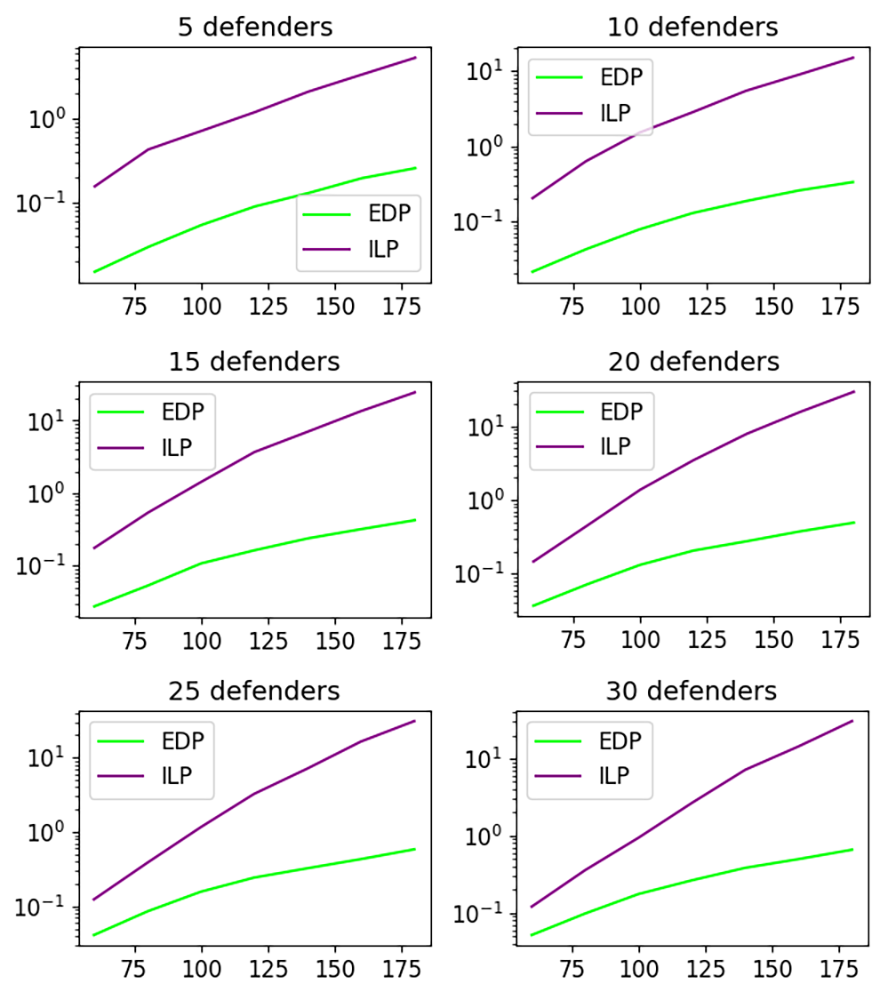
\includegraphics[width=.5\linewidth]{chapters/bd/fig/def_timecost-v.png}
    \caption[Computation time in seconds for ILP and EDP algorithms]{Computation time in seconds for ILP and EDP algorithms for $5$ to $30$ defenders and up to $200$ 
    attack events (Limit the number of events because as shown in ~\ref{fig:bd-time_cost}, 
    more events will effectively cripple ILP). \ours consistently demonstrates 1-2 magnitudes faster computation time compared with ILP.}
    \label{fig:bd-def_time_cost}
\end{figure}

\begin{figure}[h!]
    \centering
    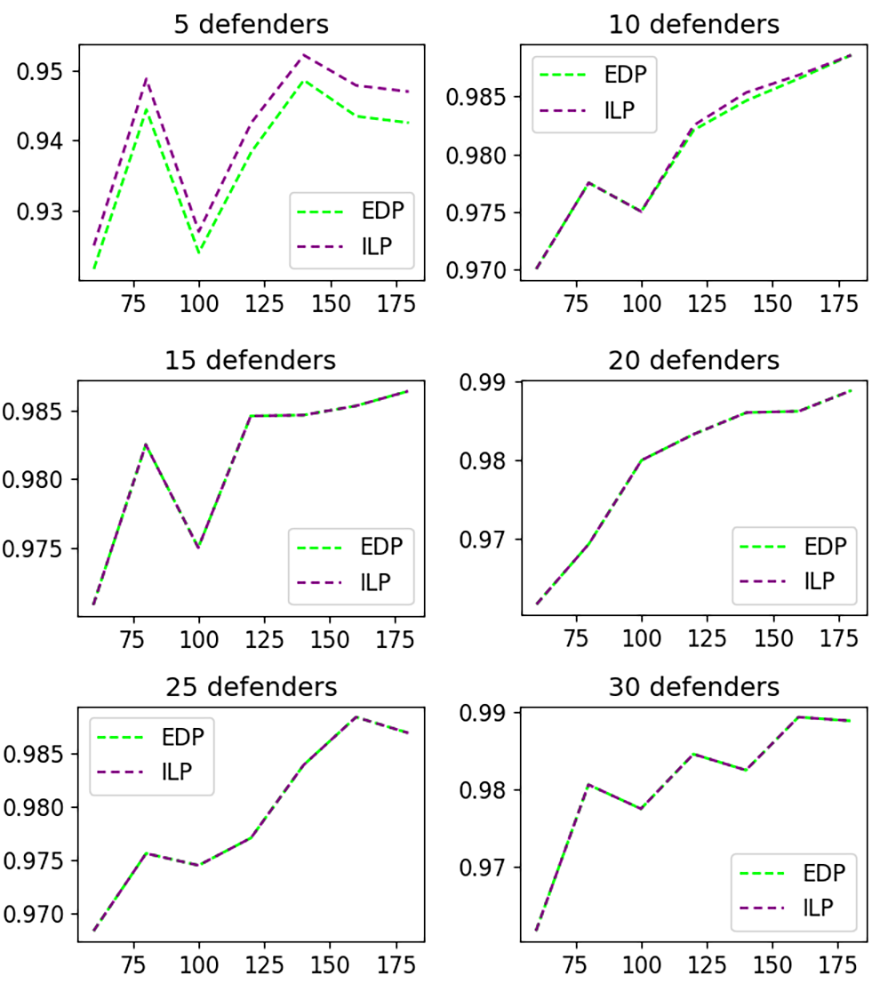
\includegraphics[width=.5\linewidth]{chapters/bd/fig/def_quality-v.png}
    \caption[Solution quality (interception rate) for the ILP and EDP]{Solution quality (interception rate) for the ILP and EDP for 5 to 30 defenders. 
    It is straightforward to observe that \ours achieves defending quality nearly identical to the optimal ILP solution (while ILP is still scalable).}
    \label{fig:bd-def_quality}
\end{figure}

As can be observed, EDP, due to its quadratic dependence on the number of defenders, consistently and significantly outperforms the ILP method in terms of computation time. At the same time, it yields virtually the same level of optimality as ILP, which guarantees that the result is optimal. 

\subsection{Impact of Defender Heterogeneity}
To explore the impact of the diversity of defender speeds on interception rate, we focus on a $5$-defender setting and to make the difference more visible, 
$\lambda$ is set to be $5\cdot k = 25$ so that the interception rate no more than 80\%. 
Here, the defender speed diversity is tested by setting the $v_{min}$ as 1, and $v_{max}$ from 1 (uniform speed) to 10, 
and then normalizing the defender speed to make them sum up to $15$ (i.e., with an average of $3.0$). 
Each data point is based on 100 runs. The result is summarized in ~\ref{fig:bd-heterogeneity}, 
from which we can observe that uniform speed $v_{max} = 1$ has the least interception rate, 
while the interception rate gets into its maximum after $v_{max}:v_{min} = 3$ or $4$. 
This suggests that heterogeneity can significantly enhance the interception rate, 
warrant the effort going into the current study (and previous study of heterogeneous defender setups). 
At the same time, as heterogeneity continues to increase, the effect becomes negligible. 
This also follows intuition: when the capability of the defenders varies too much, 
they can no longer effectively collaboratively intercept attacks. 

\begin{figure}[h!]
    \centering
    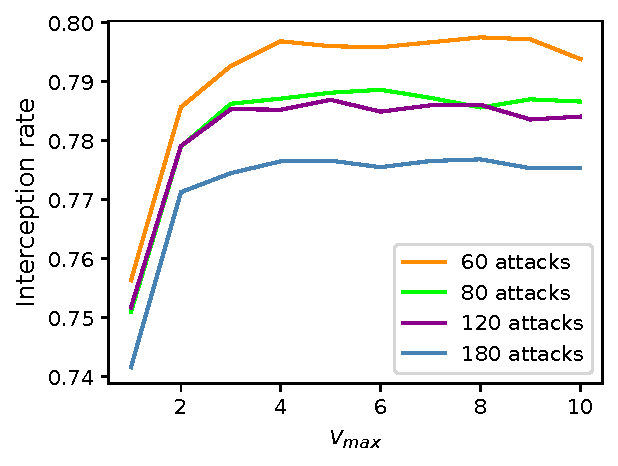
\includegraphics[width=0.5\linewidth]{chapters/bd/fig/heterogeneity.pdf}
    \caption[Solution quality (interception rate) for a different level of defender speeds diversity]{Solution quality (interception rate) for a different level of defender speeds diversity. It can be observed that the major difference happens as $v_{max}:v_{min}$ increases from $1$ to up to $4$. After that, the increase of interception rate no longer shows improvements.}
    \label{fig:bd-heterogeneity}
    \vspace{-2mm}
\end{figure}

\subsection{Impact of Attack Rate $\lambda$}
With the increase of $\lambda$ in the Poisson process for the attack sequence, 
there will be fewer attacks intercepted, 
and more defenders will be required to reach the same interception rate. 
In this regard, we test the interception rate computed using \ours for $1$ to $20$ defenders and different $\lambda$ from $1.0$ to $60.0$. 
The number of attacks is set to be $400$, and each data point represents an average of 20 runs.
~\ref{fig:bd-lambda} shows the resulting capture rate with respect to the attack rate $\lambda$ as a heat map for a different number of defenders $k$, which, unsurprisingly, suggests a gradual change as one might expect. Nevertheless, such a graph can serve as a quick reference for selecting an appropriate number defenders given an expected attack rate.

\begin{figure}[h!]
    \vspace{-2mm}
    \centering
    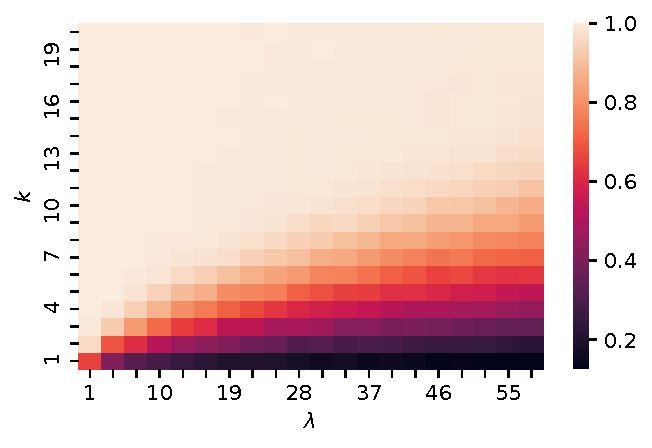
\includegraphics[width=0.5\linewidth]{chapters/bd/fig/lambda.pdf}
    \vspace{-2mm}
    \caption[Interception rate with different $\lambda$ (x-axis) and number of defenders]
    {Interception rate with different $\lambda$ (x-axis) and $k$ (y-axis, number of defenders). As one might expect, as attacks happens more frequently, holding other factors unchanged, the interception rate decreases. Similarly, holding other factors unchanged, increasing the number of defenders leads to increased interception rates.}
    \label{fig:bd-lambda}
    \vspace{-2mm}
\end{figure}

\subsection{Impact of Boundary Topology}
\ours applies to \prob with arbitrary boundary topology; we evaluated \ours on $I=[0, 1]$ (unit interval), $S^1$ (circle with a total circumference shrinked to $1$), $I^2$ (unit square), and $S^2$ (sphere with surface area of $1$) (see ~\ref{fig:bd-topology}) with $k = 5$, $v_{max} = 5$ and $\lambda$ from 1 to 200. 
The results are shown in ~\ref{fig:bd-geo}, where each data point is the average of 20 runs. 
We observe that $I$ and $S^1$ have similar difficulty to defend, with $I$ being a bit more challenging due to having boundaries. The same is observed for $I^2$ and $S^2$.
\begin{figure}[h!]
\vspace{2mm}
    \centering
    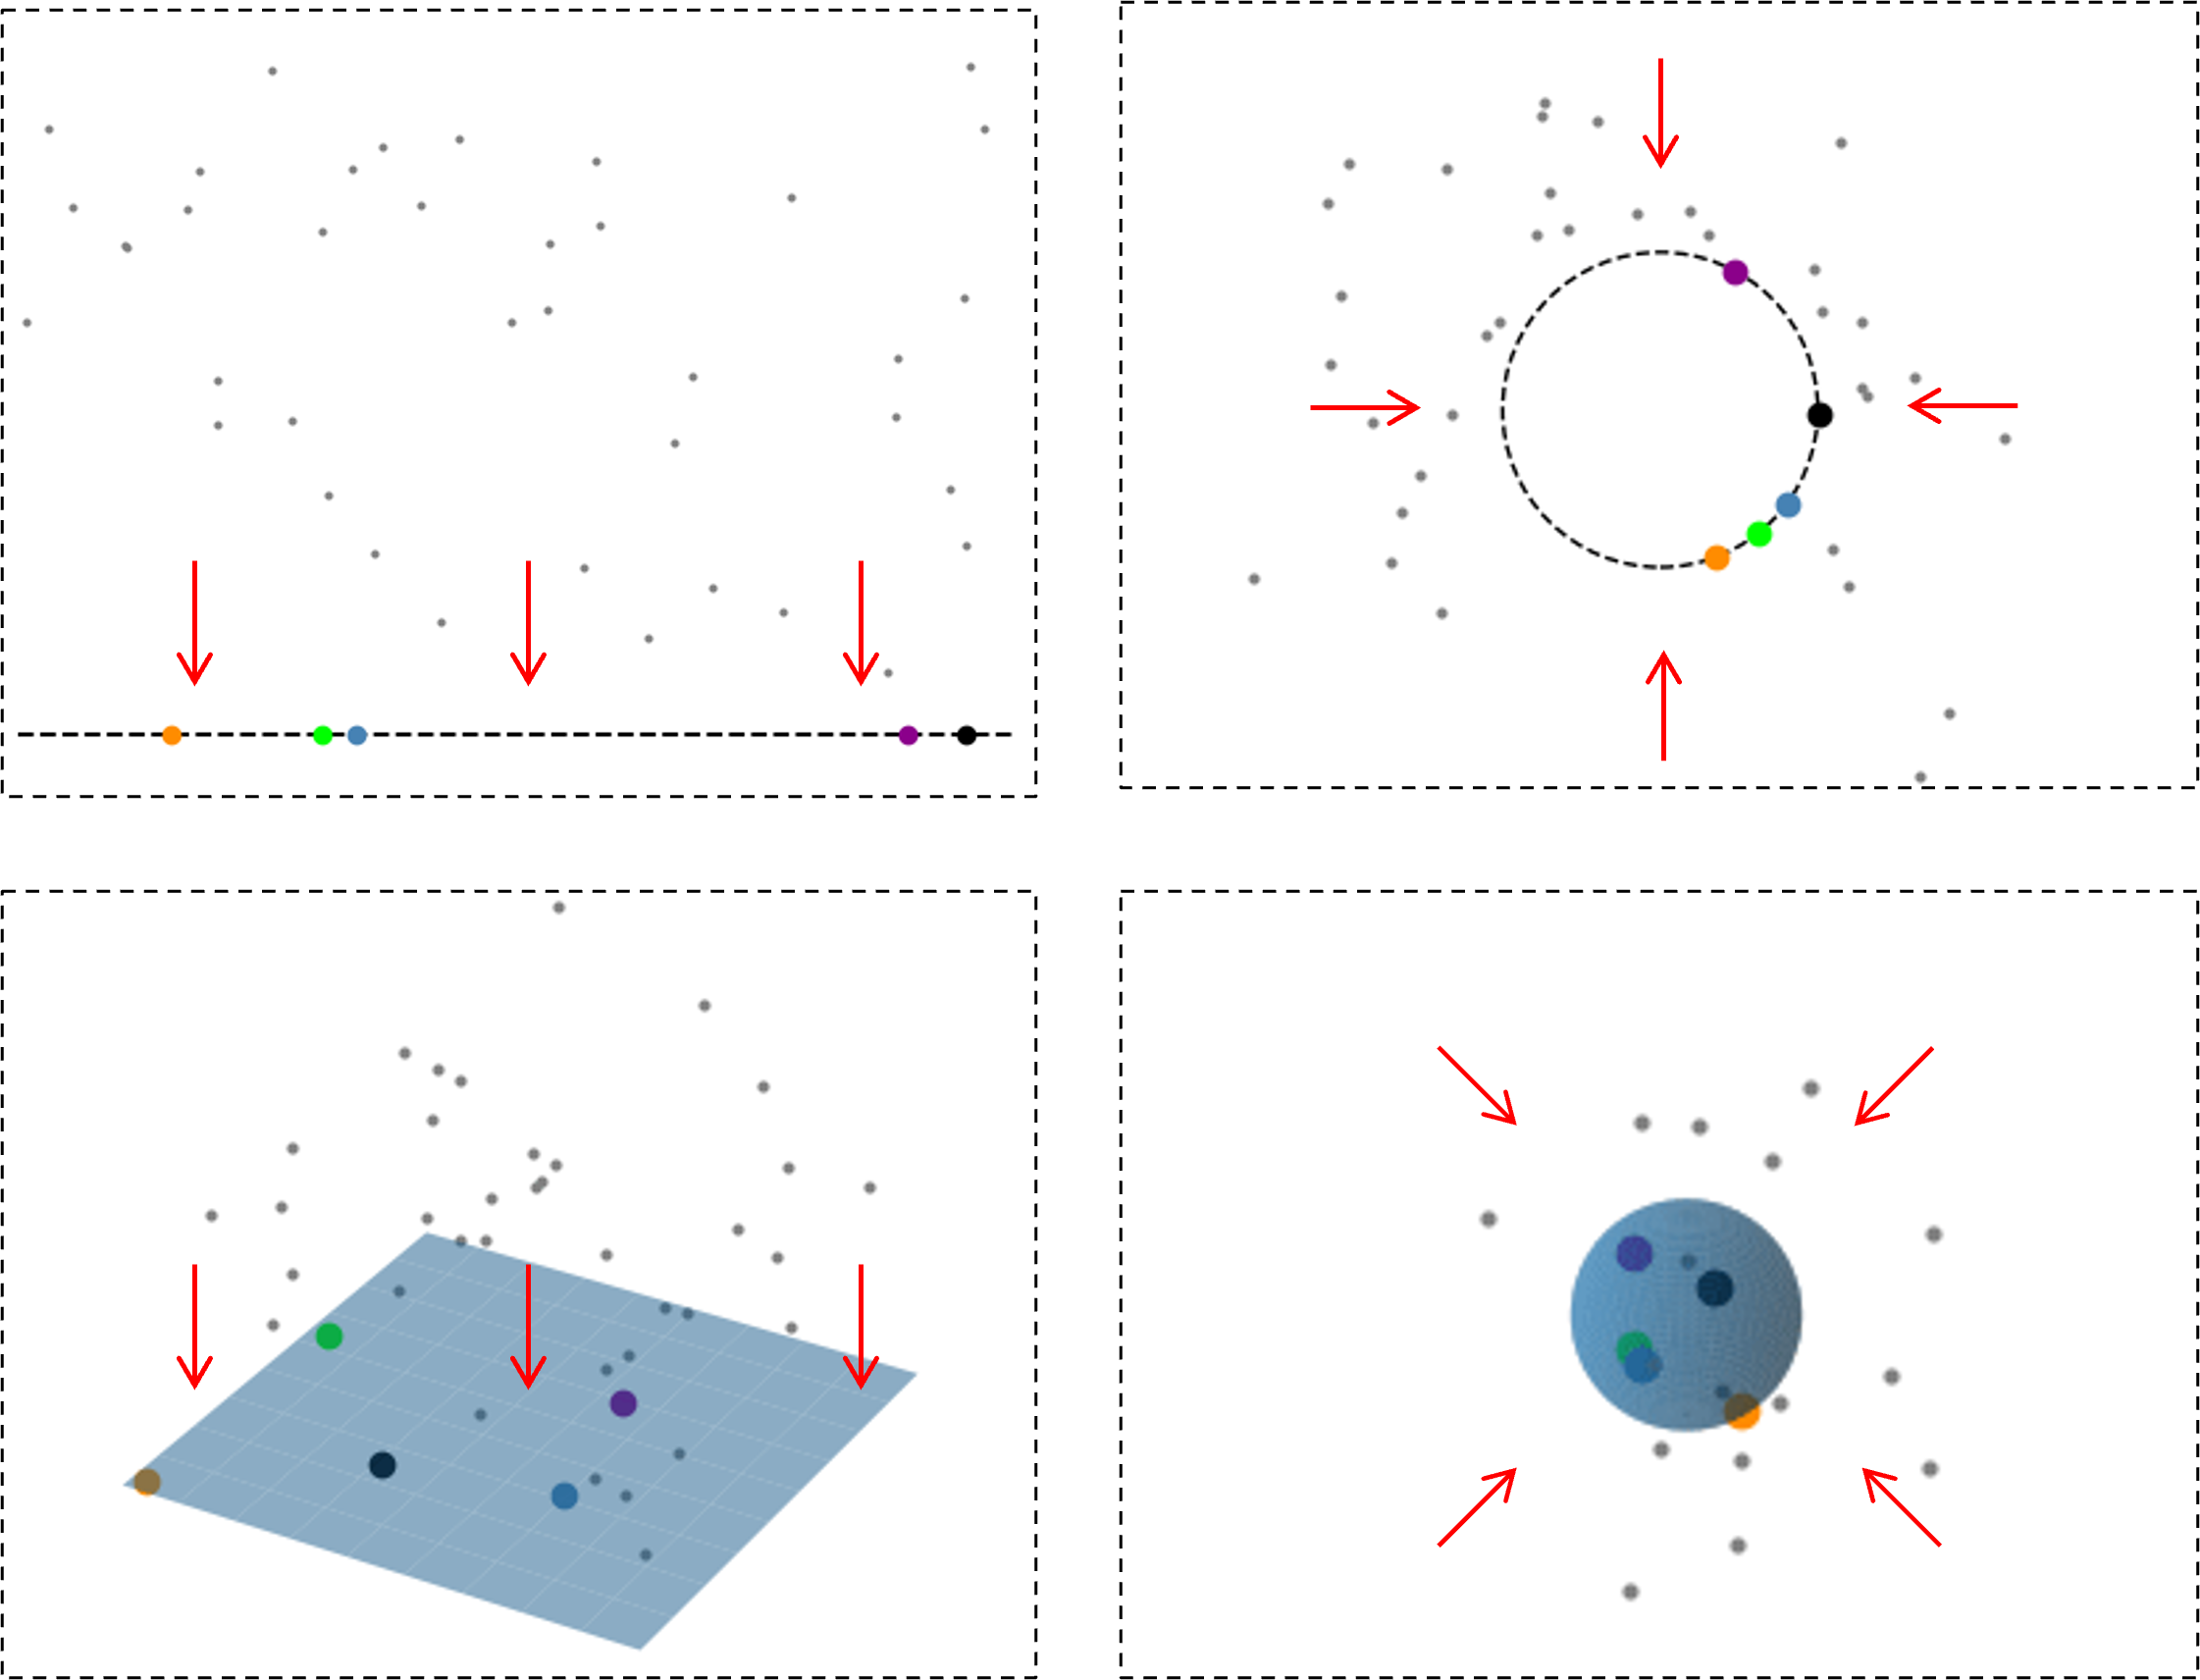
\includegraphics[width=.5\linewidth]{chapters/bd/fig/topology.png}
    \caption[\prob with boundary topologies $I$ (line segment), $S^1$ (circle), $I^2$ (unit square) and $S^2$ (sphere)]
    {\prob with boundary topologies $I$ (line segment), $S^1$ (circle), $I^2$ (unit square) and $S^2$ (sphere). The red arrows illustrate attack directions. The pictures are captured from animations of actual simulations, available at \url{https://youtu.be/x0mQD\_7RhKI}.}
    \label{fig:bd-topology}
    \vspace{-4mm}
\end{figure}

\begin{figure}[h!]
\vspace{1mm}
    \centering
    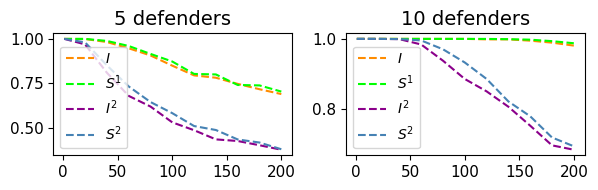
\includegraphics[width=.8\linewidth]{chapters/bd/fig/geo.png}
    \caption{Interception rate for $I$, $S^1 (\text{with length 1})$, $I^2$, $S^2 (\text{with surface area 1})$
     with different $\lambda$ from $1$ to $200$. Degradation as the number of attacks increases is as expected.}
    \label{fig:bd-geo}
\end{figure}

\subsection{Infinite Attack Stream with Finite Look-Ahead Horizon}
~\ref{alg:bd-horizon} describes an online \ours algorithm for handling the finite horizon version of the problem where the defenders only have the information about attacks in the next $T$ time frame.
Here, we present some simulation studies using the 5-defender and 400 attacks setup on an $S^1$ boundary with $v_{max} = 5$. 
~\ref{fig:bd-horizon} gives the interception rate with respect to varying defender horizons. Each data point is an average of 20 runs. 
The interception rate converges to around $1$ with a fairly short horizon, 
indicating that a long look-ahead horizon may not be necessary for effectively intercepting attacks.
\begin{figure}
    \vspace{-1mm}
    \centering
    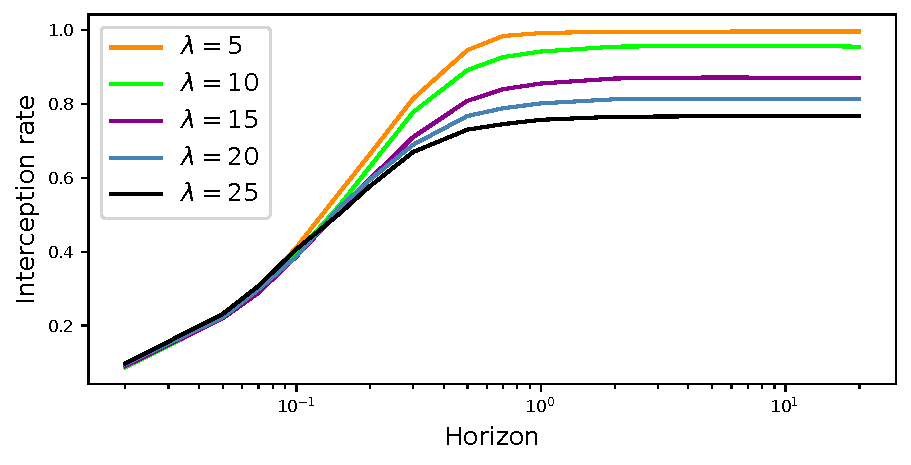
\includegraphics[width=0.6\linewidth]{chapters/bd/fig/horizon.pdf}
    \vspace{-2mm}
    \caption[Interception rate with respect to different horizons]{Interception rate with respect to different horizons (logarithmic scale). It can be observed that longer horizon allows better planning.}
    \label{fig:bd-horizon}
    \vspace{-3mm}
\end{figure}

Lastly, in ~\ref{fig:bd-solution_examples}, we provide the interception trajectories of a typical run for ILP,  \ours, and online \ours. 
%We see that, somewhat interestingly, defender switching does not happen very frequently. 
% I think the term "switching" is a bit misleading
\begin{figure}[h!]
    \vspace{1mm}
    \centering
    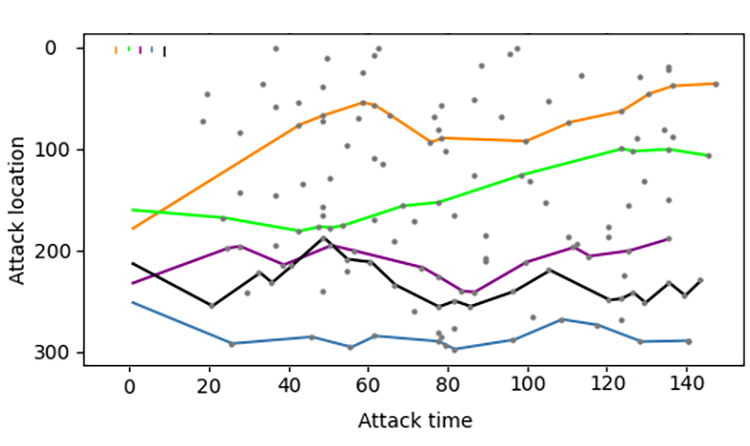
\includegraphics[width=.5\linewidth]{chapters/bd/fig/ilp_example-v.png}
    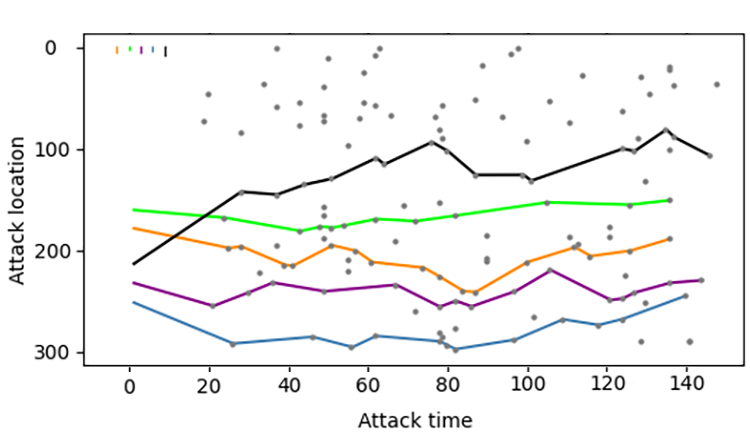
\includegraphics[width=.5\linewidth]{chapters/bd/fig/ls_example-v.png}
    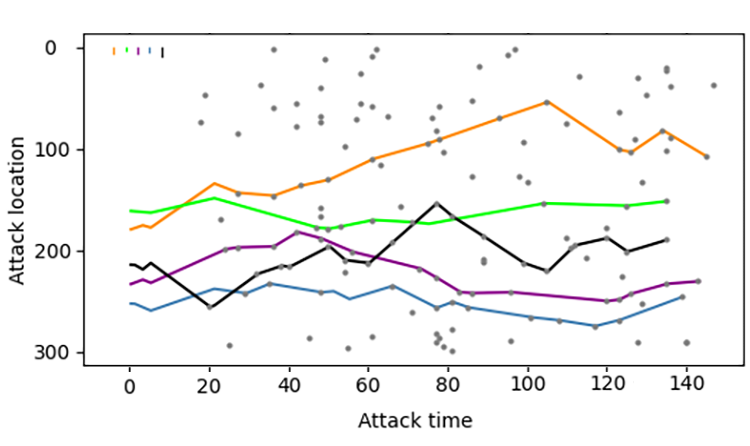
\includegraphics[width=.5\linewidth]{chapters/bd/fig/inf_horizon_example-v.png}
    \caption[The results computed by ILP, \ours, and online \ours]
    {The results computed by ILP, \ours, and online \ours with a horizon of 60, for a sequence of 140 attacks ($x$-axis is the location, $y$-axis is the time of attacks). 
    The number of captured attack events is 71, 70, and 67, respectively.}
    \label{fig:bd-solution_examples}
    \vspace{-4mm}
\end{figure}
